When conducting the research for the problem domain, We have extracted information regarding stakeholders and scope of the project. In this section we will justify our findings on technical choices regarding the deployment of the tools, design and system components. These choices are based on the requirement that is given by the product owner and the extra requirement that we think is necessary for developing a robust software.   

\subsection{Why a web application?}
Nowadays people rely heavily on using the web application. Google maps are good example of such an application, It is a very powerful software that provides to the user so many map features within a web browser, users can travel virtually within a map and can zoom for particular locations. Every time a user asks for specific information, that information is pulled dynamically into the web app.\\
 For our purpose web application is the best choice because users can access their data from various locations on any device because all data is stored online and it works on every device with a web browser. It is also safer to run an application on a web browser because It cannot interfere with programs running on the user's computer and this will lead to better performance of the machine.

\subsection{Objective}
There are various models readily available for the implementation of a web application. The choice of a specific model usually depends on the context and objectives of the project itself. Our current project entails the development of a prototype within a time constraint of 11 to 12 weeks, which persuaded us to use a full stack framework. When we would use a full stack frameword, we should be able to focus solely on techniques that allow us to perform rapid prototyping, generate quality code and provide good documentation all of which meet the clients requirements. The following features should facilitate reaching our objectives during the development phase.

\begin{enumerate}
	\item \textbf{Full stack framework}: a framework that gathers all the libraries and help us with the full development stack.
	\item \textbf{Rapid Prototyping}: enable us to convert client requirement into a rapid prototype so it can be reviewed by client and refined in the next prototype.
	\item \textbf{Scalability}: ability of a system, network, or process to handle a growing amount of work in a capable manner or its ability to be enlarged to accommodate that growth.\cite{wiki:scalability}
	\item \textbf{Reliablity}: ability of a system to function under stated conditions.
\end{enumerate}
\subsection{Project Development Methodology} % (fold)
Among several ways to develop the software Agile stands on top in practice comparing to the others (for example waterfall methodology). Scrum Agile is one of the many in agile processes, Agility (iteration) can solve the disadvantages of other development methodologies like waterfall method. In the waterfall method Development process is sequential where the whole product is tested and presented to the client only at the end; Like this if there is a mistake in the requirements, then the project has to start from scratch again correcting those requirements. Agile methodology allows for changes to be made after the initial planning and hence it is easier to add/remove features. Since Agile is based on Sprint(iteration within fixed time), at the end of each sprint, the project priorities can be evaluated by developer together with the client, This makes it possible to give his/her feedback about the product at the earlier stages.\\
Because of the aforementioned advantages of the scrum, we decided to practice scrum agile methodology for this project. The attributes and roles for people involving in the project are as follows:

\begin{enumerate}
	\item \textbf{Roles}
		\begin{itemize}
			
			\item Product Owner/Dev Team: Arnaud Hambenne
			\item Scrum master/Dev Team: Soheil Jahanshahi
			\item Client: TU Delft Library(Babak Dehghanpour , Nicoleta Nastase )
			\item Coach: Alberto Bacchelli
		\end{itemize}
	\item \textbf{\color{red}{TODO}}	
\begin{itemize}
		\item Sprint : one week iteration
		\item Sprint planning meeting: to set highest priority features for each sprint 
		\item Sprint reflections report: to evaluate the estimated effort with actual effort and to discuss the hurdles by the end of each sprint.
		\item Daily Scrum meeting: time-boxed 15 minutes
		\item Sprint Review Meeting: 15 to 20 minutes, meeting with clients to receive their feedback on the product.
		
\end{itemize} 
\end{enumerate}
\subsection{Architectural Model : MVC}
A design pattern is important to write re-usable and maintainable code. For the Virtual assistant application is best to divide the application into three interconnected parts to separate internal representation of information from information that is presented to users or accepted by them\cite{wiki:mvc}. Such a Design is called MVC pattern which consist of three separate parts namely Model, View and Controller.
\begin{figure}[h]
\centering
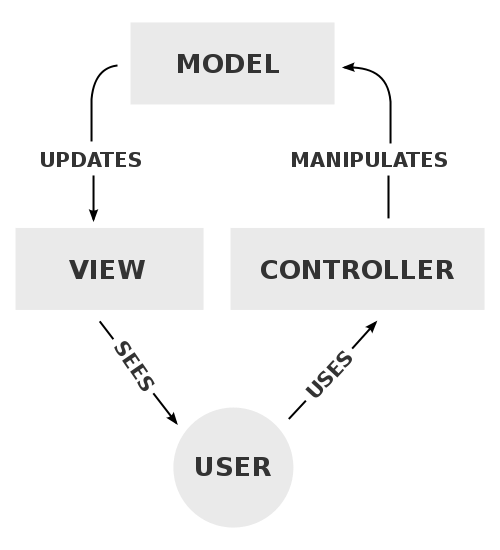
\includegraphics[scale=0.3]{./img/MVC.PNG}
\caption{\small{model,view and controller that are interconnected by directed edges}}
\label{mvc}
	
\end{figure}

As shown in fig \ref{mvc} , MVC will give the application power to separate the classes which are used typically in a database from the user interface; that is necessary to render the model to the user. also controller will act as a brain of the application. controller decides what the user input was and how the model needs to change as a result of that input\cite{codinghorror},controller then respond back to the user by calling resulting view.

\subsection{Choice of framework}
For choosing suitable web application framework we have conducted some  constraint for ourselves to benchmark various popular existing frameworks which is proven in production. Our first criteria was choosing a framework which is based on either Java, Scala, Javascript. With this we have narrowed down our choices to search for the suitable framework. After Analyzing popular frameworks such as \href{https://grails.org/}{Grails}, \href{https://vaadin.com/home}{Vaadin}, \href{https://www.playframework.com/}{Play!} and \href{http://projects.spring.io/spring-framework/}{Spring}. We finally selected two candidates to benchmark them. We boiled down our choices between Spring framework and Play! framework.\\
\subsubsection{Benchmarking}
 below table shows comparison of these two frameworks with constraint that we have settled:\\\\

\begin{center}
	

\begin{tabular}{ |l||l|p{7cm}|p{6cm}|  }
 \hline
 \multicolumn{4}{|c|}{\textbf{Benchmark Table}} \\
 \hline
 ~ & \textbf{Constraint} & \textbf{Play! Framework} & \textbf{Spring Framework}\\
 \hline
 1   & Development Principles & Convention over configuration,Don't repeat yourself,Test-driven development & Convention over configuration,Don't repeat yourself,Test-driven development ,Domain Driven Design   \\
 \hline
 2 & Design pattern & Model-View-Controller,Dependency-injection,Active-Record,DAO,Actors & Model-View-Controller,Dependency-injection,Domain-Driven-Design \\
 \hline
 3 &Operating System & Cross-Platform&  Cross-Platform\\
 \hline
 4 &Programming Language & Java, Scala &  Java\\
 \hline
 5& Database  & MySQL,PostgreSQL,MongoDB,Oracle,SQLite,HBase,H2-database,Resis& Microsoft-BI,MYSQL,PostgreSQL,Oracle,SQLite,IBM-DB2,JDBC-Compatible,MongoDB,Microsoft-SQL-Server,Taradata,Cassandra\\
 \hline
 6&   Database model  & NoSQL,Relational,Object-Relational & Document-Oriented,Graph-Oriented,Multidimensional,NoSQL,Relational,Object-Relational,XML Database\\
 \hline
 7&   Documentation level & Excellent&Excellent\\
 \hline
 8&   Programming paradigm  & OOP,Functional,Concurrency Oriented&Aspect-Oriented,OOP\\
 \hline
 9&   Cloud Platform Support  & Heroku,Clever Cloud,Amazon EC2,Cloud Bee,OpenShift,digital Ocean,playframework Cloud & Open Shift,Heroku,Amazon EC2,AppHarbor,CloudBee\\
 \hline
 10&   Annotatiuon support & YES & YES\\
 \hline
 11&   Scalability & YES&YES\\
 \hline
\end{tabular}
\end{center}

The result of Benchmarking showed that there are actually not much of a difference between these two frameworks. Finally we decided to use Play!Framework for this project.

\subsection{Play! Framework}


% \begin{enumerate}
% 	\item User(Client) interaction with web(Asynchronous vs sync)
% 	\item Distributed application structure(client/server)
% 	\item Scalability is the ability of a system, network, or process to handle a growing amount of work in a capable manner or its ability to be enlarged to accommodate that growth.
% 	\item Build systems
% 	\item Databases(need more research)
% 	\item Continuous Integration
% \end{enumerate}
% \subsubsection{Synchronous Vs Asynchronous}
% \subsubsection{Server-Side Rendering Vs Client/Server}
% \subsubsection{Vertical Scalability Vs. Horizontal Scalability}
% \subsubsection{sbt Vs. Maven}
% \subsubsection{mongodb vs nosql vs mysql vs postgres}
% \subsubsection{Template}
% \subsubsection{Testing}
% \subsubsection{Jenkins}
% \subsubsection{frameworks}


